\chapter{Day 4: loops \& functions}

\section{Summary of topics}
% Summarize the topics from the “listen” segment of the day (150 – 250 words)

The topics for today where loops and functions. Loops make it possible to repeat a part of code multiple times, avoiding code duplication. There are two types of loops, while loops and for loops. The wile loop takes on the following structure:

\begin{codebox}{example 4.1}
    \begin{lstlisting}
while (statement) {
    // code that will repeat as long as the statement is true
}
    \end{lstlisting}
\end{codebox}

The while starts by checking if the statement is \texttt{true} or \texttt{false}. If the statement is \texttt{true} the code inside the block is executed once. The statement is checked again and while it remains \texttt{true}, the code is repeated. Important to note is that if the statement is false to begin with, the code is never executed and if the statement is always true, the program will get stuck in an endless loop.

Often times a variable is used which is updated inside of the loop. Eventually this will result in the statement becoming \texttt{false}. See example 4.2. The counter starts at 0, and inside the loop is increased by 1 each time until it becomes 10 at which point the statement will be false and the loop stops.

\begin{codebox}{example 4.1}
    \begin{lstlisting}
int counter = 0; 
while (counter < 10) { 
    counter = counter + 1 // or counter++; 
}
    \end{lstlisting}
\end{codebox}

A for loop puts all of this logic together, making it better suited for this purpose. It takes on the following structure:

\begin{codebox}{example 4.3}
    \begin{lstlisting}
while (init; statement; update) {
    // code that will repeat as long as the statement is true
}
    \end{lstlisting}
\end{codebox}

Here, the \texttt{init} statement is executed first, then the \texttt{statement} is evaluated and if the test is true, the code inside the block is executed. After that, the \texttt{update} is executed and the process is repeated. In example 4.4 a real example is demonstrated. This code behaves exactly the same as example 4.3.

\begin{codebox}{example 4.4}
    \begin{lstlisting}
while (int counter = 0; counter < 10; counter++) {
    // code that will repeat as long as the statement is true
}
    \end{lstlisting}
\end{codebox}

Finally it was also demonstrated that you can use loops within each other (nested loops). This can be used to fill a grid with dots for example.

\medskip

The second topic where functions. These are self-contained modules that can be seen as an factory you give an instruction. The instructions are given through parameters. Some functions can also return a value using the \texttt{return} keyword. They are useful to make code easier to read, modify and expand. Let's take a look at two types:

\begin{codebox}{example 4.5}
    \begin{lstlisting}
void function(type1 parameter1, type2 parameter2) {
    // code that uses parameter1 and 2 to do something
}

int function(type1 parameter1, type2 parameter2) {
    // code that uses parameter1 and 2 to do something and return an integer
    return integerVariable;
}
    \end{lstlisting}
\end{codebox}

The first function takes in two parameters and uses these to do something (but return nothing). The second function does the same, but will return an integer value which can be used further in the program. Both functions can be called using \texttt{function(parameter1, parameter2)}.

\newpage

\section{Challenge description: Etch a Sketch}
% A description of that day’s challenge describing what the assignment was, what you tried to achieve and how you applied the topics from the “listen” segment. include instruction on how to use is and Include screenshots/screen captures. (150 – 250 words)

The assignment for today was to create an interactive image. My goal was to create a digital \textit{Etch a Sketch}. A Etch a Sketch is a drawing toy which has two dials which can be used to move a stylus inside of the toy. The styles etches into the back of the screen which creates a drawing. Shaking the toy will remove the image so it can be used again. In \cref{fig: etch a sketch} the toy is shown.

\begin{figure}[H]
    \centering
    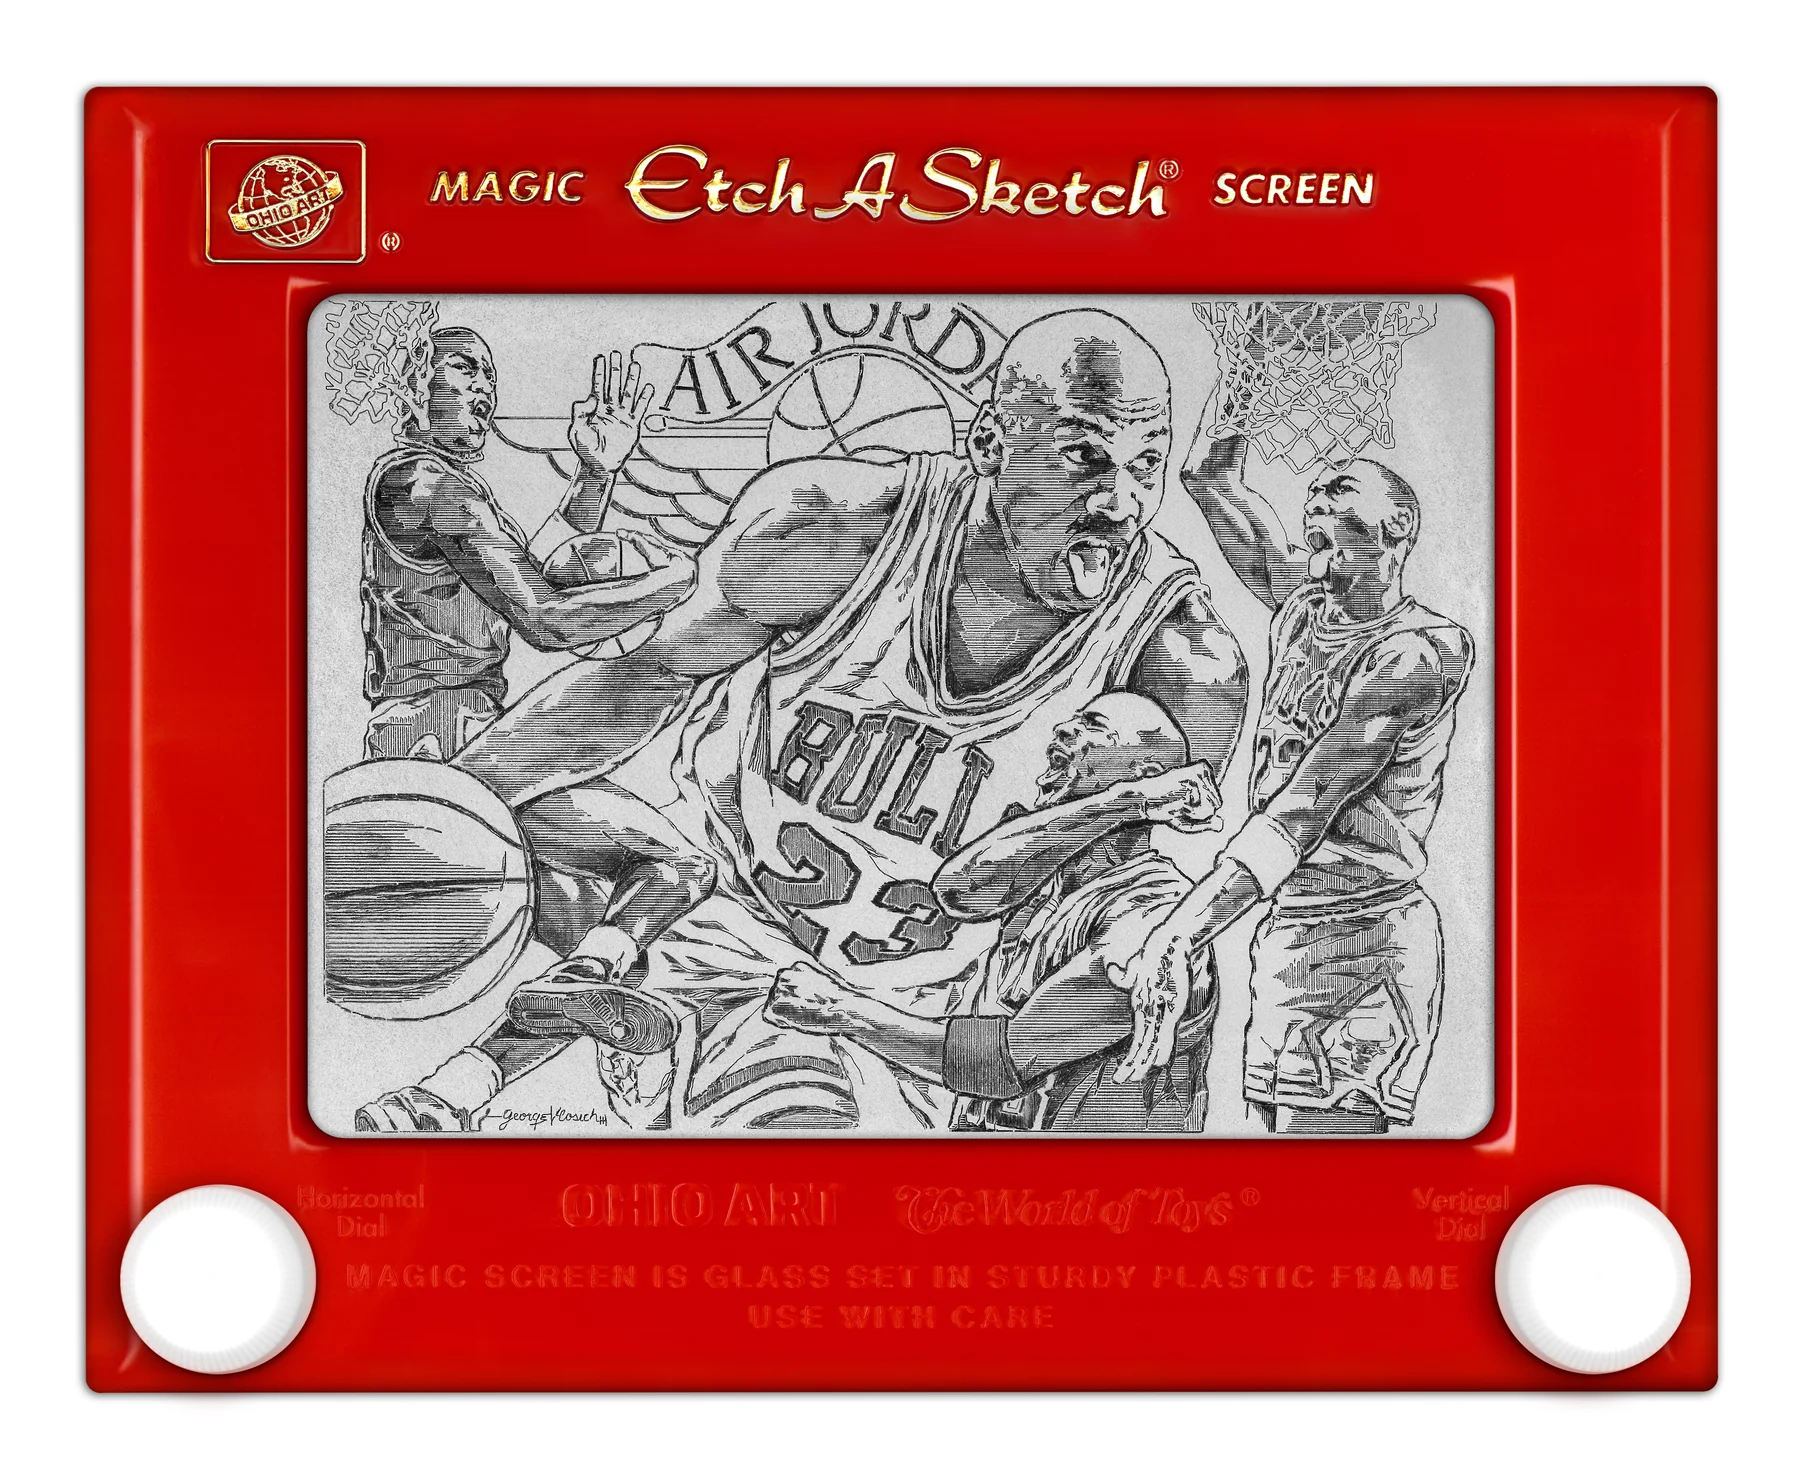
\includegraphics[width = 0.5 \textwidth]{Figures/day_4/etch_a_sketch.png}
    \caption{A typical Etch a Sketch}
    \label{fig: etch a sketch}
\end{figure}

In the code, I used a nested loop in the \texttt{render()} method of the \texttt{Canvas} class in order to draw each of the squares which make up the `screen' of the device. I used plenty of functions to create reusable code. In particular, the \texttt{Dial} class could be used as a generic dial in any application. Finally, I used the methods \texttt{mousePressed()} and \texttt{mouseDragged()} in order to make the dial respond to clicking and dragging the mouse.

\medskip

The result is shown in \cref{fig: my etch a sketch}. Once the program is launched, you can click and hold the dial to start rotating it. By making circulair motions while holding the mouse button you can rotate the dial both directions. The location of the `stylus' is shown in white. The left dial controls the horizontal direction of the stylus and the right dial the vertical direction.

\begin{figure}[H]
    \centering
    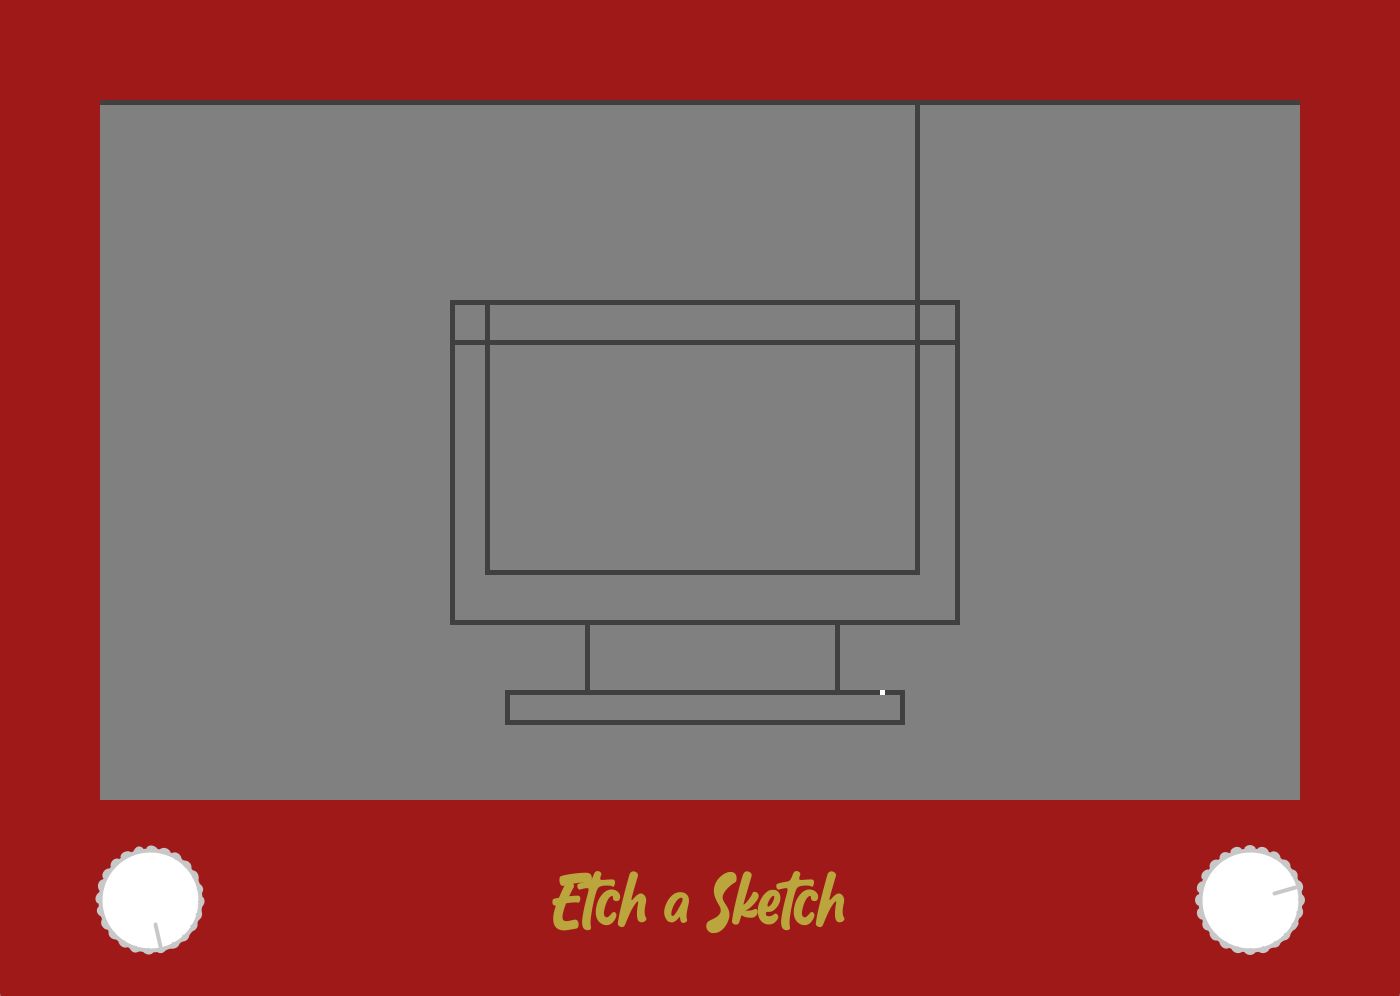
\includegraphics[width = 0.5 \textwidth]{Figures/day_4/my_etch_a_sketch.png}
    \caption{My digital Etch a Sketch}
    \label{fig: my etch a sketch}
\end{figure}

I tried to draw a computer monitor, I challenge you to do better :).